\documentclass[10pt]{beamer}

%PACKAGES
\usetheme{metropolis}
\usepackage{appendixnumberbeamer}
\usepackage{booktabs}
\usepackage[scale=2]{ccicons}
\usepackage{pgfplots}
\usepgfplotslibrary{dateplot}
\usepackage{xspace}
\usepackage{listings}
\usepackage{graphicx}


%SETTINGS
\definecolor{codegreen}{rgb}{0.5,0.6,0.5}
\definecolor{codegray}{rgb}{0.5,0.5,0.5}
\definecolor{codeorange}{rgb}{1,0.5,0}
\definecolor{backcolour}{rgb}{0.95,0.95,0.95}

\lstdefinestyle{mystyle}{
    backgroundcolor=\color{backcolour},   
    commentstyle=\itshape\color{codegreen},
    keywordstyle=\bfseries\color{codeorange},
    numberstyle=\tiny\color{codegray},
    stringstyle=\color{blue},
    basicstyle=\footnotesize,
    breaklines=true,
    breakatwhitespace=true,
    captionpos=b,                    
    keepspaces=true,                 
    numbers=left,
    numbersep=3pt,                  
    showspaces=false,                
    showtabs=false,                  
    tabsize=2,
    language=R,
    identifierstyle=\color{black},
    xleftmargin=-3pt,
}

\lstset{style=mystyle} 

\title{Spectral Indices for Algae Bloom evaluation}
\subtitle{Course of monitoring ecosystem changes and functioning}
\date{1st February 2023}
\author{Serena Negroni}

\begin{document}
\maketitle

\begin{frame}{Table of contents}
  \setbeamertemplate{section in toc}[sections numbered]
  \tableofcontents[]
\end{frame}

\section{Methods}

\begin{frame}{Study area}
Lake Erie - Great Lakes, North America \\
5th October 2011
  \begin{figure}
  \begin{minipage}{.53\textwidth}
  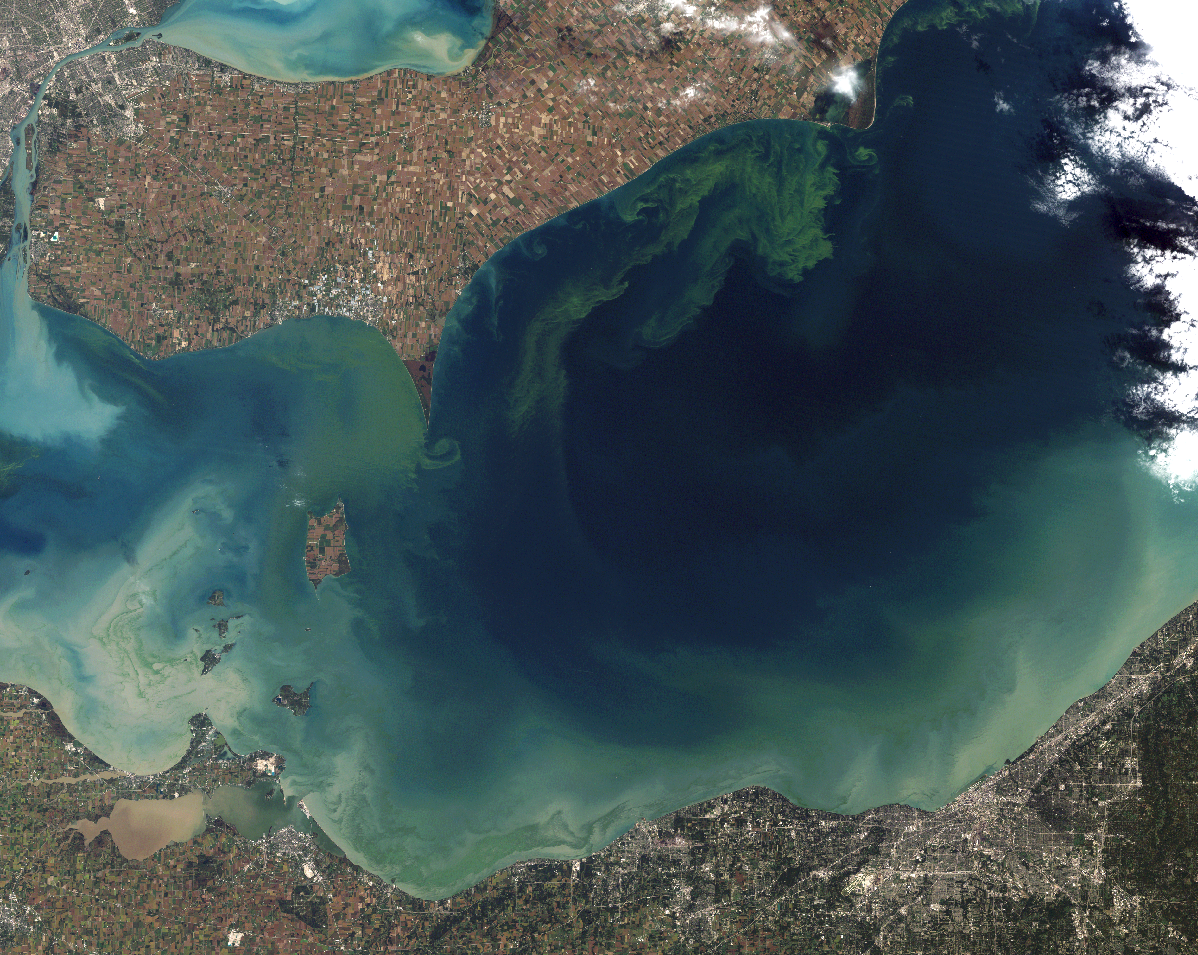
\includegraphics[width=.99\textwidth]{images/lakeerie_tm5_2011278_geo.png}
  \caption{Landsat 5, 30 m resolution image.}
  \end{minipage}
  \begin{minipage}[t]{.43\textwidth}
    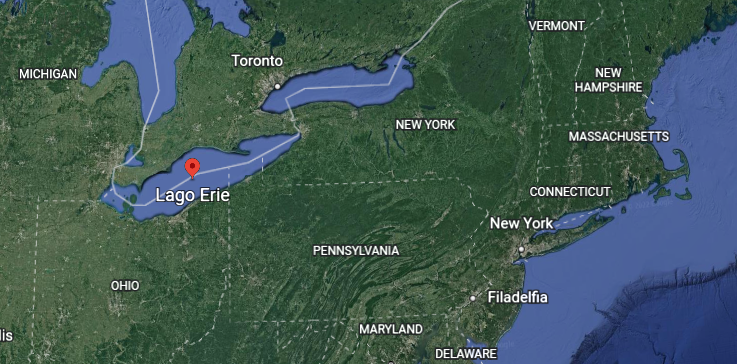
\includegraphics[width=.99\textwidth]{images/lake_out.png}
   \caption{Google Earth view.}   
  \end{minipage}
\end{figure}  
\end{frame}

\subsection{Satellite image}

\begin{frame}{Landsat 5}
Sensor: Thematic Mapper \\
Spectral bands used:
\begin{table}[h]
    \begin{tabular}{c|c|l}
    \toprule
    \midrule
  Bands & Wavelengths [$\mu m$] & Name \\
    \midrule
    1  & 0.45-0.52 &  Visible Blue\\
    2 & 0.52-0.60 & Visible Green\\ 
    3 & 0.63-0.69 & Visible Red\\
    4 & 0.76-0.90 & Near Infrared (NIR)\\
    5 & 1.55-1.75 & Short-Wave Infrared (SWIR) \\
    \midrule
    \bottomrule
\end{tabular}
\end{table}
\end{frame}

\begin{frame}[fragile]{Create the image}
\begin{lstlisting}[language = R]
#useful library
library(rgdal)  library(RStoolbox)  library(rasterdiv)

#load layers that create the image
blue <- raster("LT05_L1TP_019031_20111005_20200820_02_T1_B1.TIF") 
green <- raster("LT05_L1TP_019031_20111005_20200820_02_T1_B2.TIF") 
red <- raster("LT05_L1TP_019031_20111005_20200820_02_T1_B3.TIF") 
nir <- raster("LT05_L1TP_019031_20111005_20200820_02_T1_B4.TIF") 
swir <- raster("LT05_L1TP_019031_20111005_20200820_02_T1_B5.TIF") 

#rasteStack of all bands
file <- stack(blue, green, red, nir, swir)

#cut the image to zoom on the region of interest
#extention of the original image: 283185, 430005, 4514385, 4732515  
boundary <- raster(xmn = 365000, xmx = 430000 , ymn = 4600000,  ymx = 4680000)
\end{lstlisting}
\end{frame}

\begin{frame}[fragile]{}
\begin{lstlisting}[firstnumber=17]
#geographical subset of the original image
image <- crop(file, boundary)
plotRGB(image, r = 3, g = 2, b = 1, stretch = "lin")
\end{lstlisting}
\begin{figure}
\centering
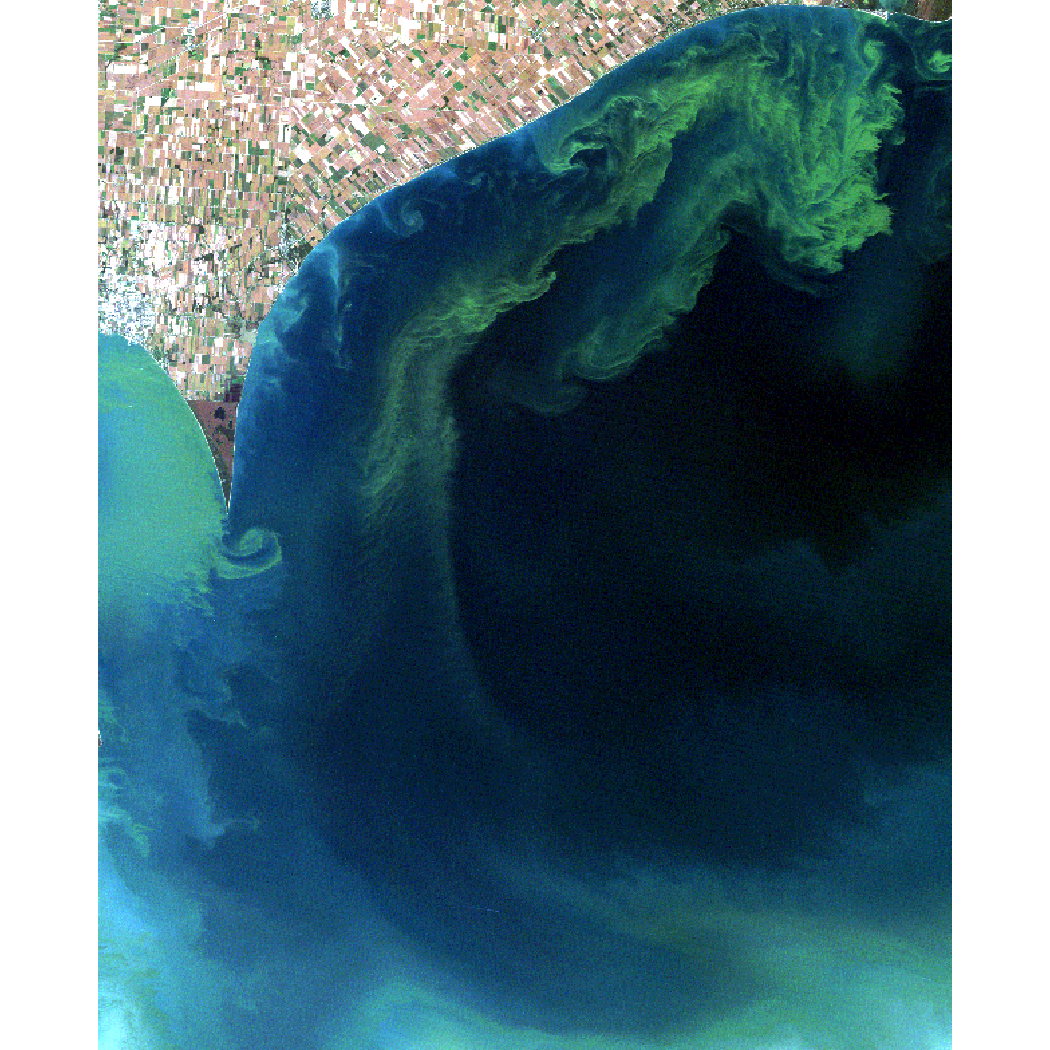
\includegraphics[width=.7\textwidth]{images/rgbTrue.pdf}
\end{figure}  
\end{frame}

\subsection{Masking}

\begin{frame}[fragile]{Masking}
\begin{lstlisting}[firstnumber=20]
#infrared image
rgb_lw <- stack(red, nir, swir)
boundary <- raster( xmn = 365000, xmx = 430000 , ymn = 4600000, ymx = 4680000)
image_lw <- crop(rgb_lw, boundary)

plot(image_lw, xaxt = 'n', yaxt = 'n', main = c( "Red_Band_3", "NIR_Band_4", "SWIR_Band_5"))
\end{lstlisting}

  The image produced by band 5 is the one with the greatest contrast between land and sea.

\begin{lstlisting}[firstnumber=26]
#create the mask 
swir_image <- crop(swir, boundary)
swir_image[swir_image > 11] <- NA
\end{lstlisting}
\end{frame}

\begin{frame}{Infrared image}
\begin{figure}
\centering
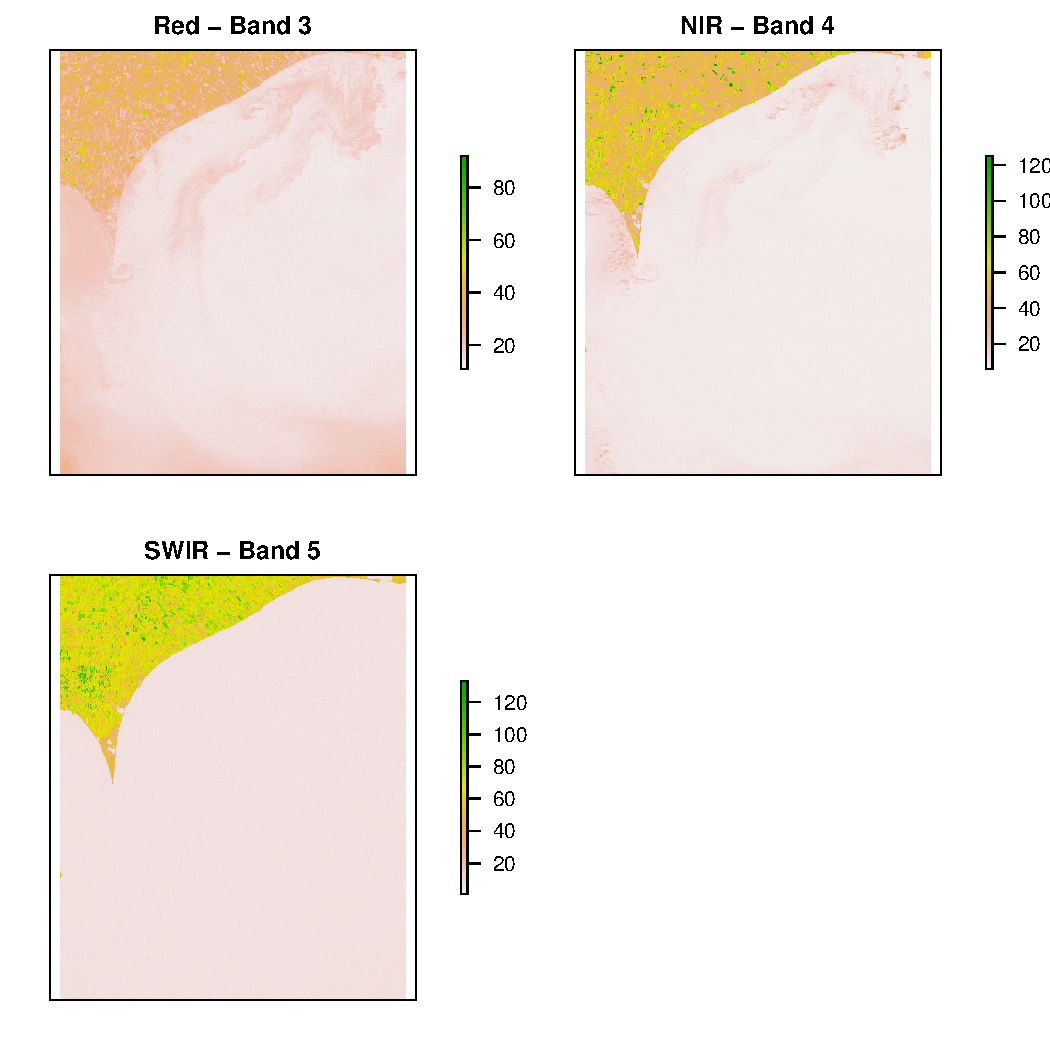
\includegraphics[width=.7\textwidth]{images/rgbFalse.pdf}
\end{figure}  
\end{frame}

\begin{frame}{Land mask}
   \centering
    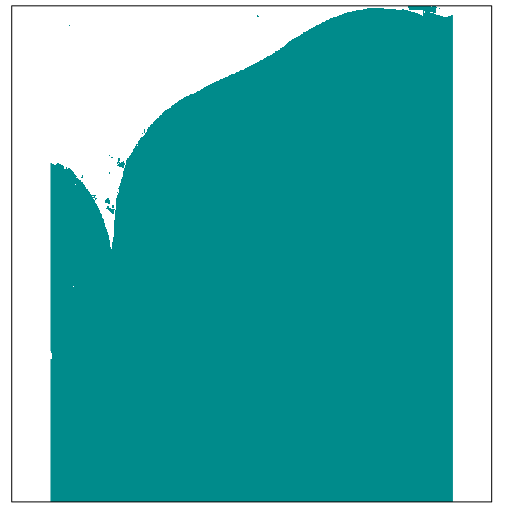
\includegraphics[width=0.6\textwidth]{images/mask.png} 
\end{frame}


\begin{frame}[fragile]{}
\begin{lstlisting}[firstnumber = 29]
#apply the mask
image_masked <- mask(image, mask = swir_image) 

plotRGB(image_masked, r = 3, g = 2, b = 1, stretch = "lin")
legend("top", legend = NA, title = expression(bold("RGB_True_Color")), bty = "n", cex = 1.3)

plotRGB(image_masked, r = 4, g = 3, b = 2, stretch = "lin") 
legend("top", legend = NA, title = expression(bold("RGB_False_Color")), bty = "n", cex = 1.3)
\end{lstlisting}
 \begin{figure}
    \centering
    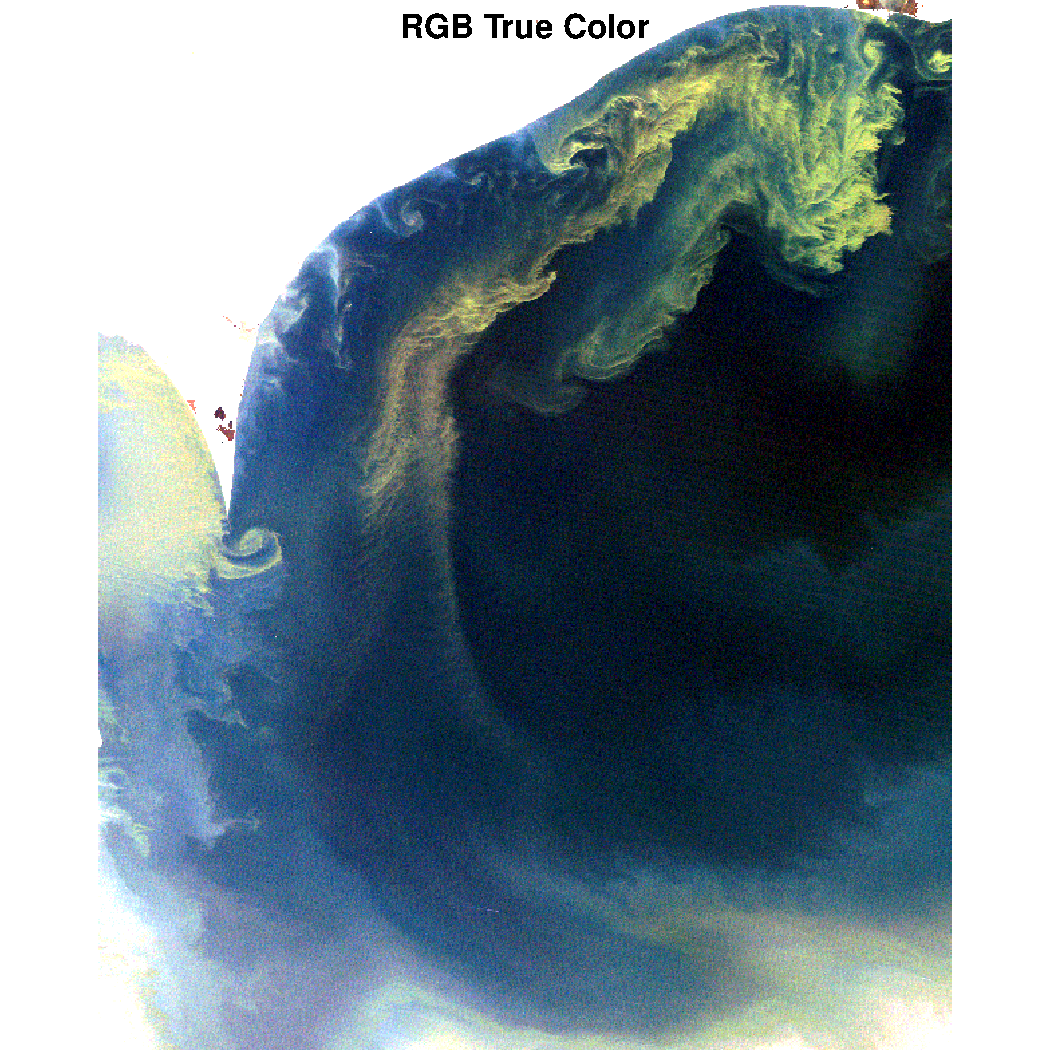
\includegraphics[width=0.45\textwidth]{images/masked_rgb.pdf}
    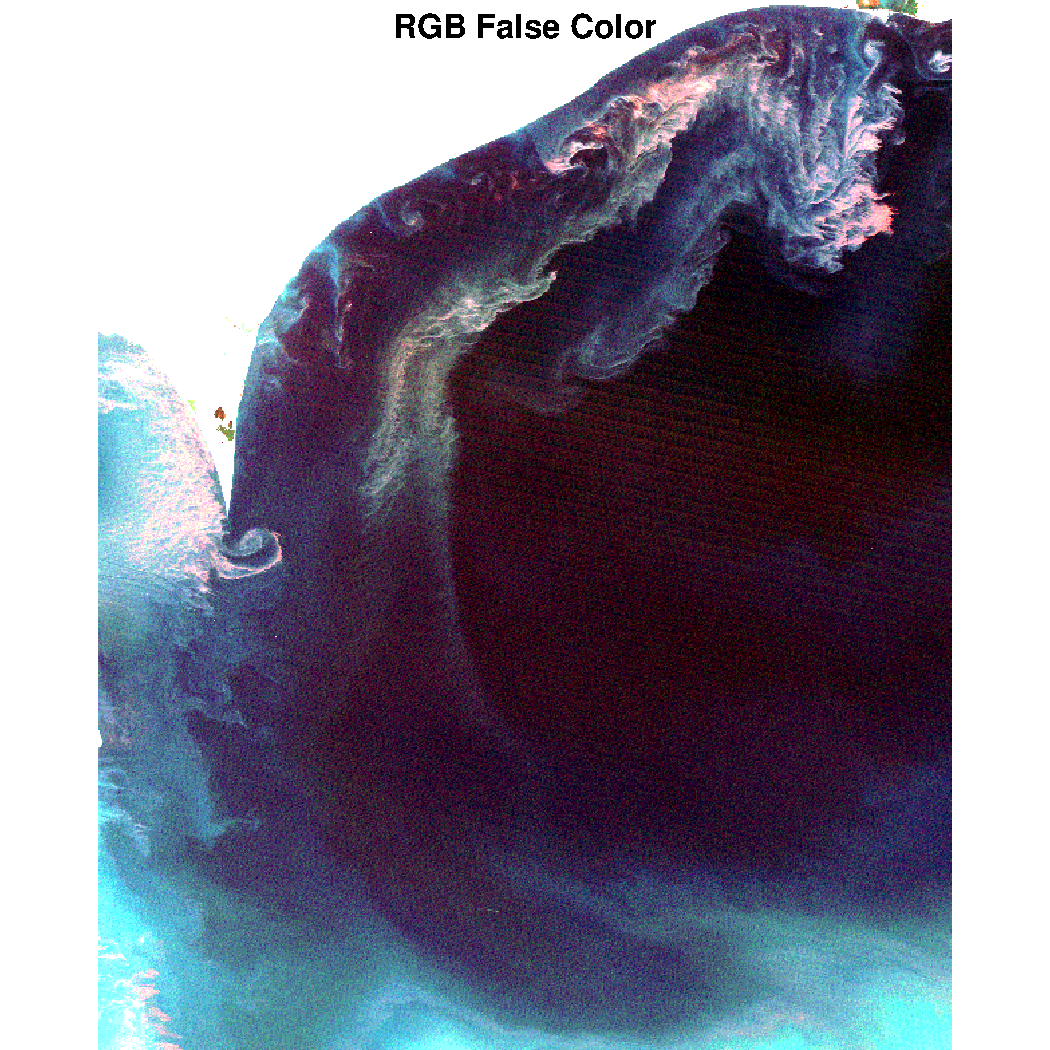
\includegraphics[width=0.45\textwidth]{images/masked_false.pdf}
\end{figure}
%Contrast increased
\end{frame}

\section{Spectral indices}

\begin{frame}[fragile]{Difference Vegetation Index (DVI)}
\begin{lstlisting}[firstnumber = 37]
#specify color scheme
library(RColorBrewer)
colors <- colorRampPalette(c('darkblue', 'yellow', 'red', 'black'))(100)

dvi <- image_masked[[4]] - image_masked[[3]]  
plot(dvi, main = "DVI", col = colors)
\end{lstlisting}
\begin{minipage}{0.55\textwidth}
\begin{figure}
\centering
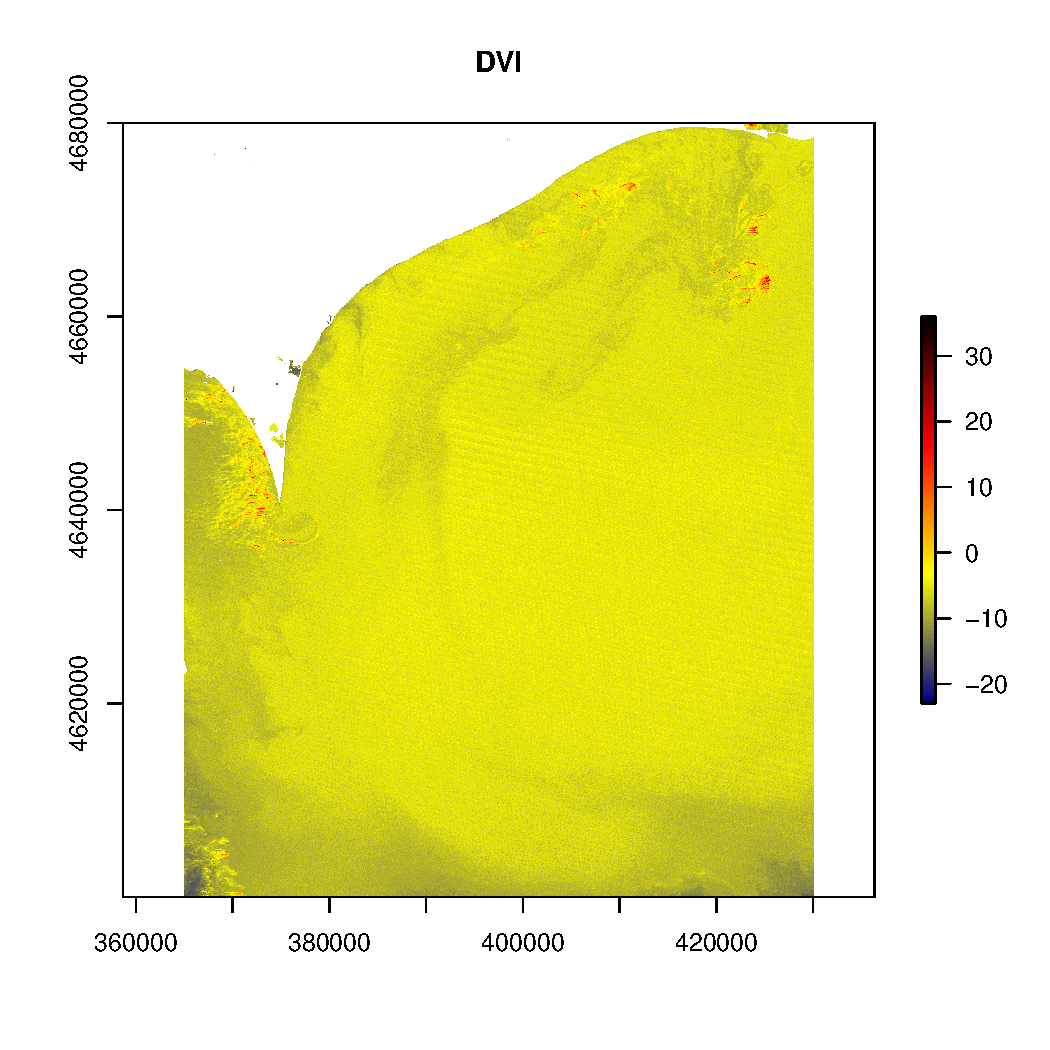
\includegraphics[width=.9\textwidth]{images/dvi.pdf}
\end{figure}   
\end{minipage}
\begin{minipage}[b]{0.4\textwidth}
\centering \Large DVI = NIR - Red
\end{minipage} 
\end{frame}

\begin{frame}[fragile]{Normalized DVI (NDVI)}
\begin{lstlisting}[firstnumber = 43]
ndvi <- ((image_masked[[4]] - image_masked[[3]]) / (image_masked[[4]] + image_masked[[3]]))

plot(ndvi, main = "NDVI", col = colors)
\end{lstlisting}
\begin{minipage}{.6\textwidth}
\begin{figure}[ht]
\centering
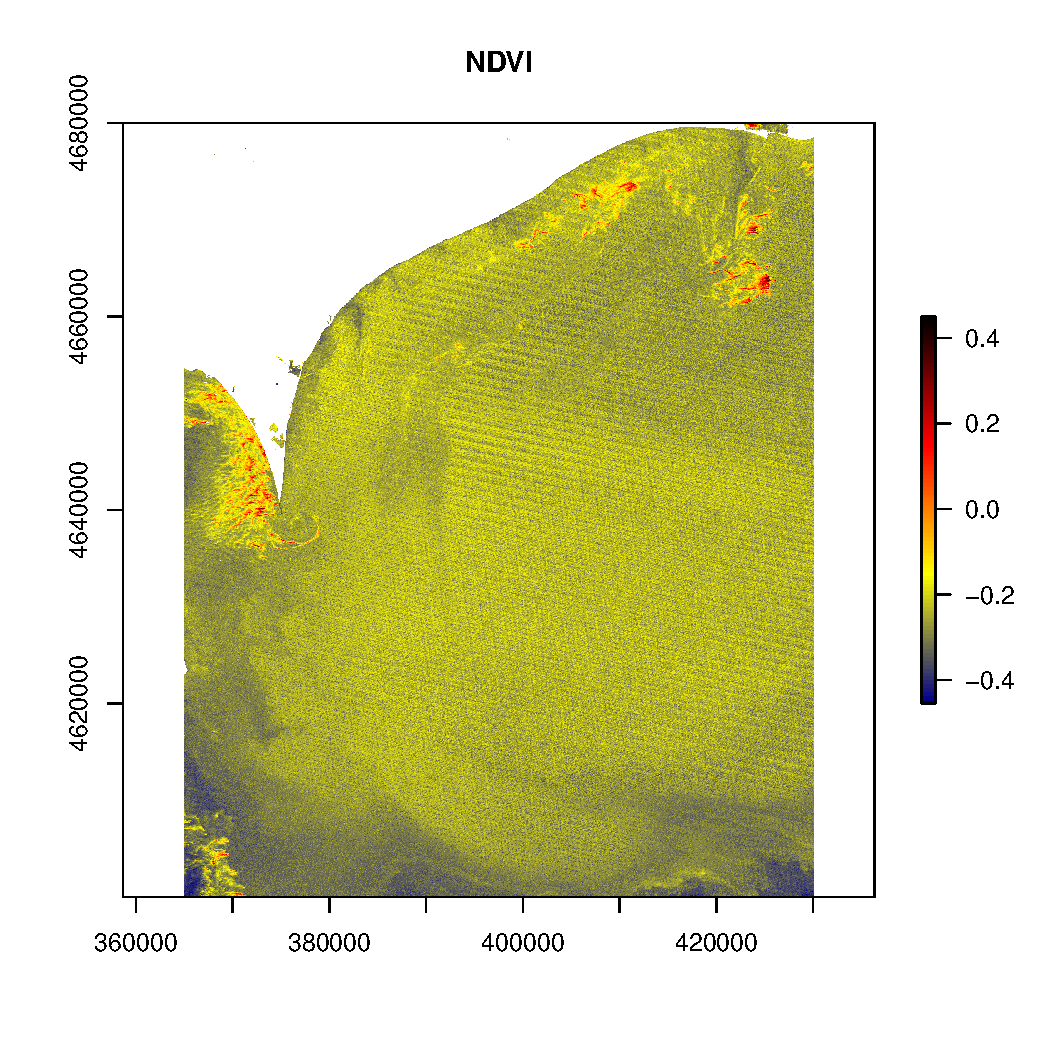
\includegraphics[width=0.9\textwidth]{images/ndvi.pdf}
\end{figure}  
\end{minipage}
 \begin{minipage}[b]{.30\textwidth}
 \centering
\Large NDVI = \Large $\frac{\text{NIR} - \text{Red}}{\text{NIR} + \text{Red}}$  
 \end{minipage}
\end{frame}

\begin{frame}[fragile]{Surface Algae Bloom Index (SABI)}
\begin{lstlisting}[firstnumber = 46]
sabi <- (image_masked[[4]] - image_masked[[3]]) / (image_masked[[1]] + image_masked[[2]])

plot(sabi, main = "SABI", col = colors)
\end{lstlisting}
\begin{minipage}{.6\textwidth}
\begin{figure}[ht]
\centering
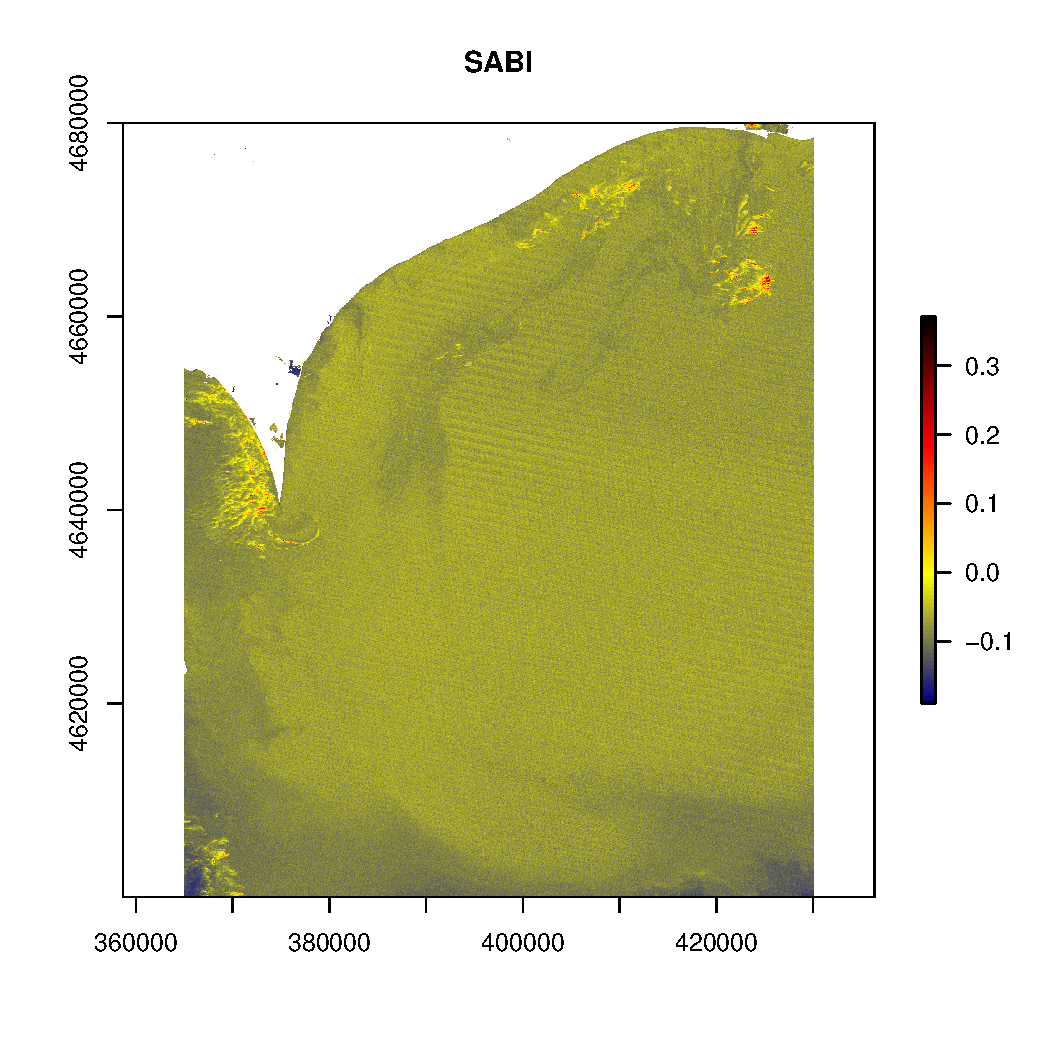
\includegraphics[width=0.9\textwidth]{images/sabi.pdf}
\end{figure}  
\end{minipage}
 \begin{minipage}[b]{.35\textwidth}
 \centering 
\large SABI = \Large $\frac{\text{NIR} - \text{Red}}{\text{Blue} + \text{Green}}$ 
\end{minipage}
\end{frame}

\begin{frame}[fragile]{Floatin Algae Index (FAI)}
\begin{lstlisting}[firstnumber = 49]
fai <- image_masked[[4]] - image_masked[[3]] - (image_masked[[5]] - image_masked[[3]])*((0.83 - 0.66) / (1.65 - 0.66))

plot(fai, main = "FAI", col = colors)
\end{lstlisting}
\begin{minipage}{.6\textwidth}
\begin{figure}
\centering
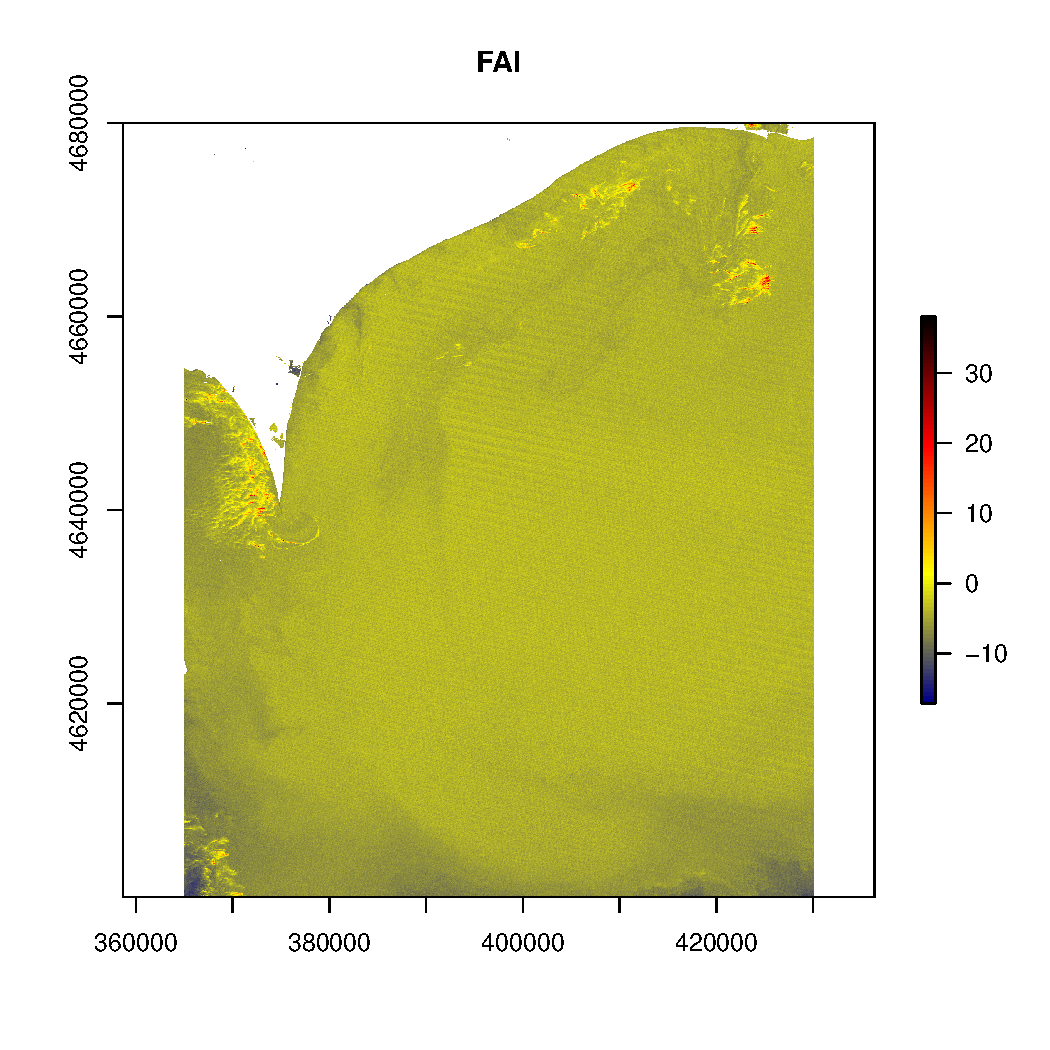
\includegraphics[width=0.9\textwidth]{images/fai.pdf}
\end{figure}  
\end{minipage}
 \begin{minipage}[b]{.35\textwidth}
\centering
\large FAI = \large NIR - Red - (SWIR - Red)*$R_{\lambda}$ \\
\vspace{0.5cm}
 with $\large R_{\lambda} = \frac{\lambda_{\text{NIR}} - \lambda_{\text{Red}}}{\lambda_{\text{SWIR}} - \lambda_{\text{Red}}}$ 
\end{minipage}
\end{frame}

\subsection{Comparisons among indeces}
\begin{frame}{Comparisons}
\begin{figure}
    \centering
    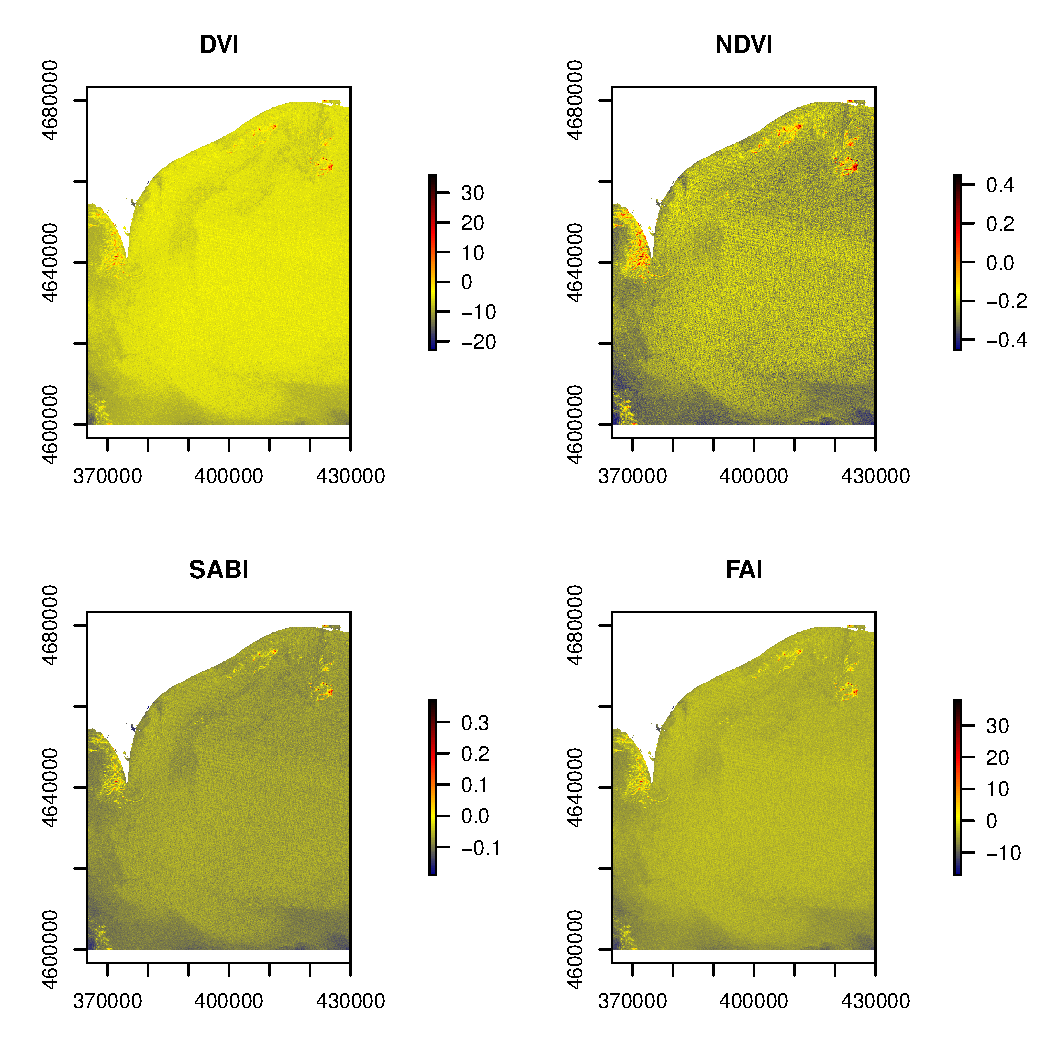
\includegraphics[width=0.75\textwidth]{images/confronto.pdf}
\end{figure}  
\end{frame}

\begin{frame}[fragile]{ggplot Graphs}
\begin{lstlisting}[firstnumber = 52]
library(ggplot2)
#create a data frame with the indices (raster)
index <- stack(dvi, ndvi, sabi, fai)
dat <- as.data.frame(index)
#delete NAN
dat <- na.omit(dat)

#histograms
p1 <- ggplot(dat, aes(x = layer.1)) + 
     geom_histogram(color = "black", fill = "chartreuse3", alpha = 0.4, lwd = 0.5) + labs(title = "DVI_distribution", x = "Value", y = "Frequency")

#densities
d1 <- ggplot(dat, aes(x = layer.1)) + 
     geom_density(color = "chartreuse3", fill = "chartreuse3", alpha = 0.25) + labs(title = "DVI_density", x = "Value", y = "Density")
\end{lstlisting}   
Same procedure for the other 3 indices. Then use \textit{\textbf{library(patchwork)}} to combine them in one image: \textit{\textbf{(p1 + p2) / (p3 + p4)}}.
\end{frame}

\begin{frame}{Histograms}
\begin{figure}
    \centering
    \includegraphics[width=\textwidth]{images/hist_gg.pdf}
\end{figure}  
\end{frame}

\begin{frame}{Densities}
\begin{figure}
    \centering
    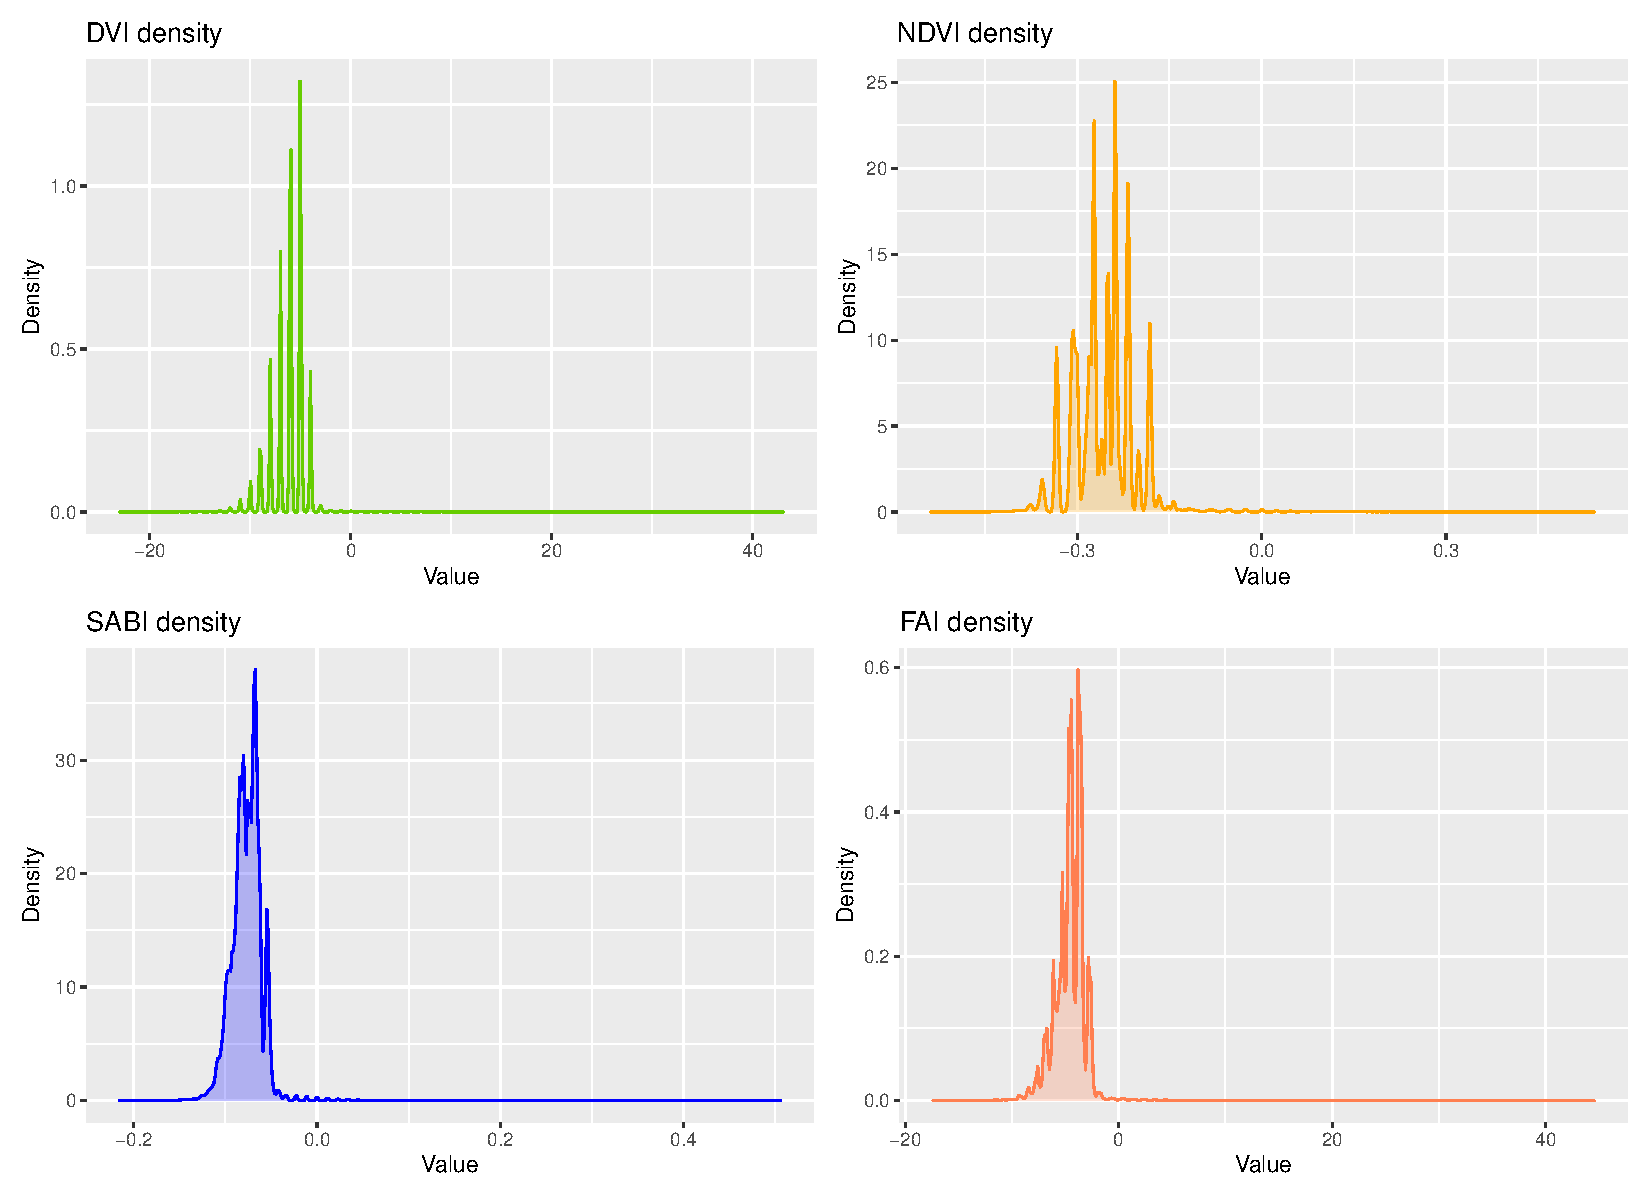
\includegraphics[width=\textwidth]{images/density.pdf}
\end{figure}  
\end{frame}

\subsection{Chlorophyll estimation}

\begin{frame}[fragile]{Chlorophyll Index (CI)}
\begin{lstlisting}[firstnumber = 66]
ci <- image_masked[[4]] / image_masked[[2]] - 1

plot(ci, main = "CI", col = colors)    
\end{lstlisting}
 \begin{minipage}{0.6\textwidth}
 \begin{figure}
\centering
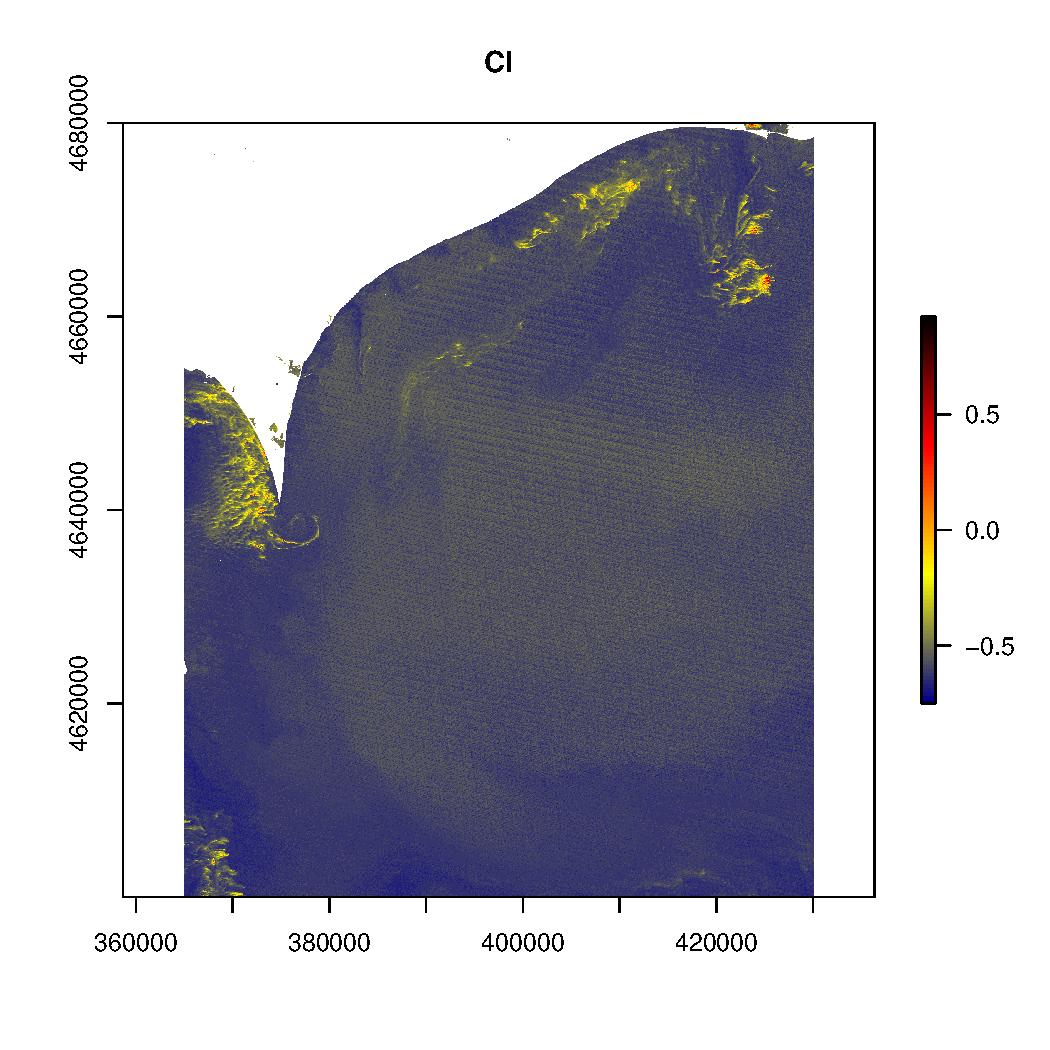
\includegraphics[width=0.9\textwidth]{images/ci.pdf} 
\end{figure}
\end{minipage} 
\begin{minipage}[b]{.35\textwidth}
\centering
\Large CI = \Large $\frac{NIR}{Green}$ - 1
\end{minipage}
\end{frame}

\begin{frame}[fragile]{Chlorophyll estimation}
\small Comparison between positive SABI and FAI values and CI
\begin{lstlisting}[firstnumber = 69]
#copy raster's indices
sabi_pos <- sabi
fai_pos <- fai
ci_pos <- ci

#select only positive value for SABI and FAI and CI > -0.5
sabi_pos[sabi_pos < 0] <- NA
fai_pos[fai_pos < 0] <- NA
ci_pos[ci_pos < -0.5] <- NA
\end{lstlisting}
\begin{figure}
    \centering
    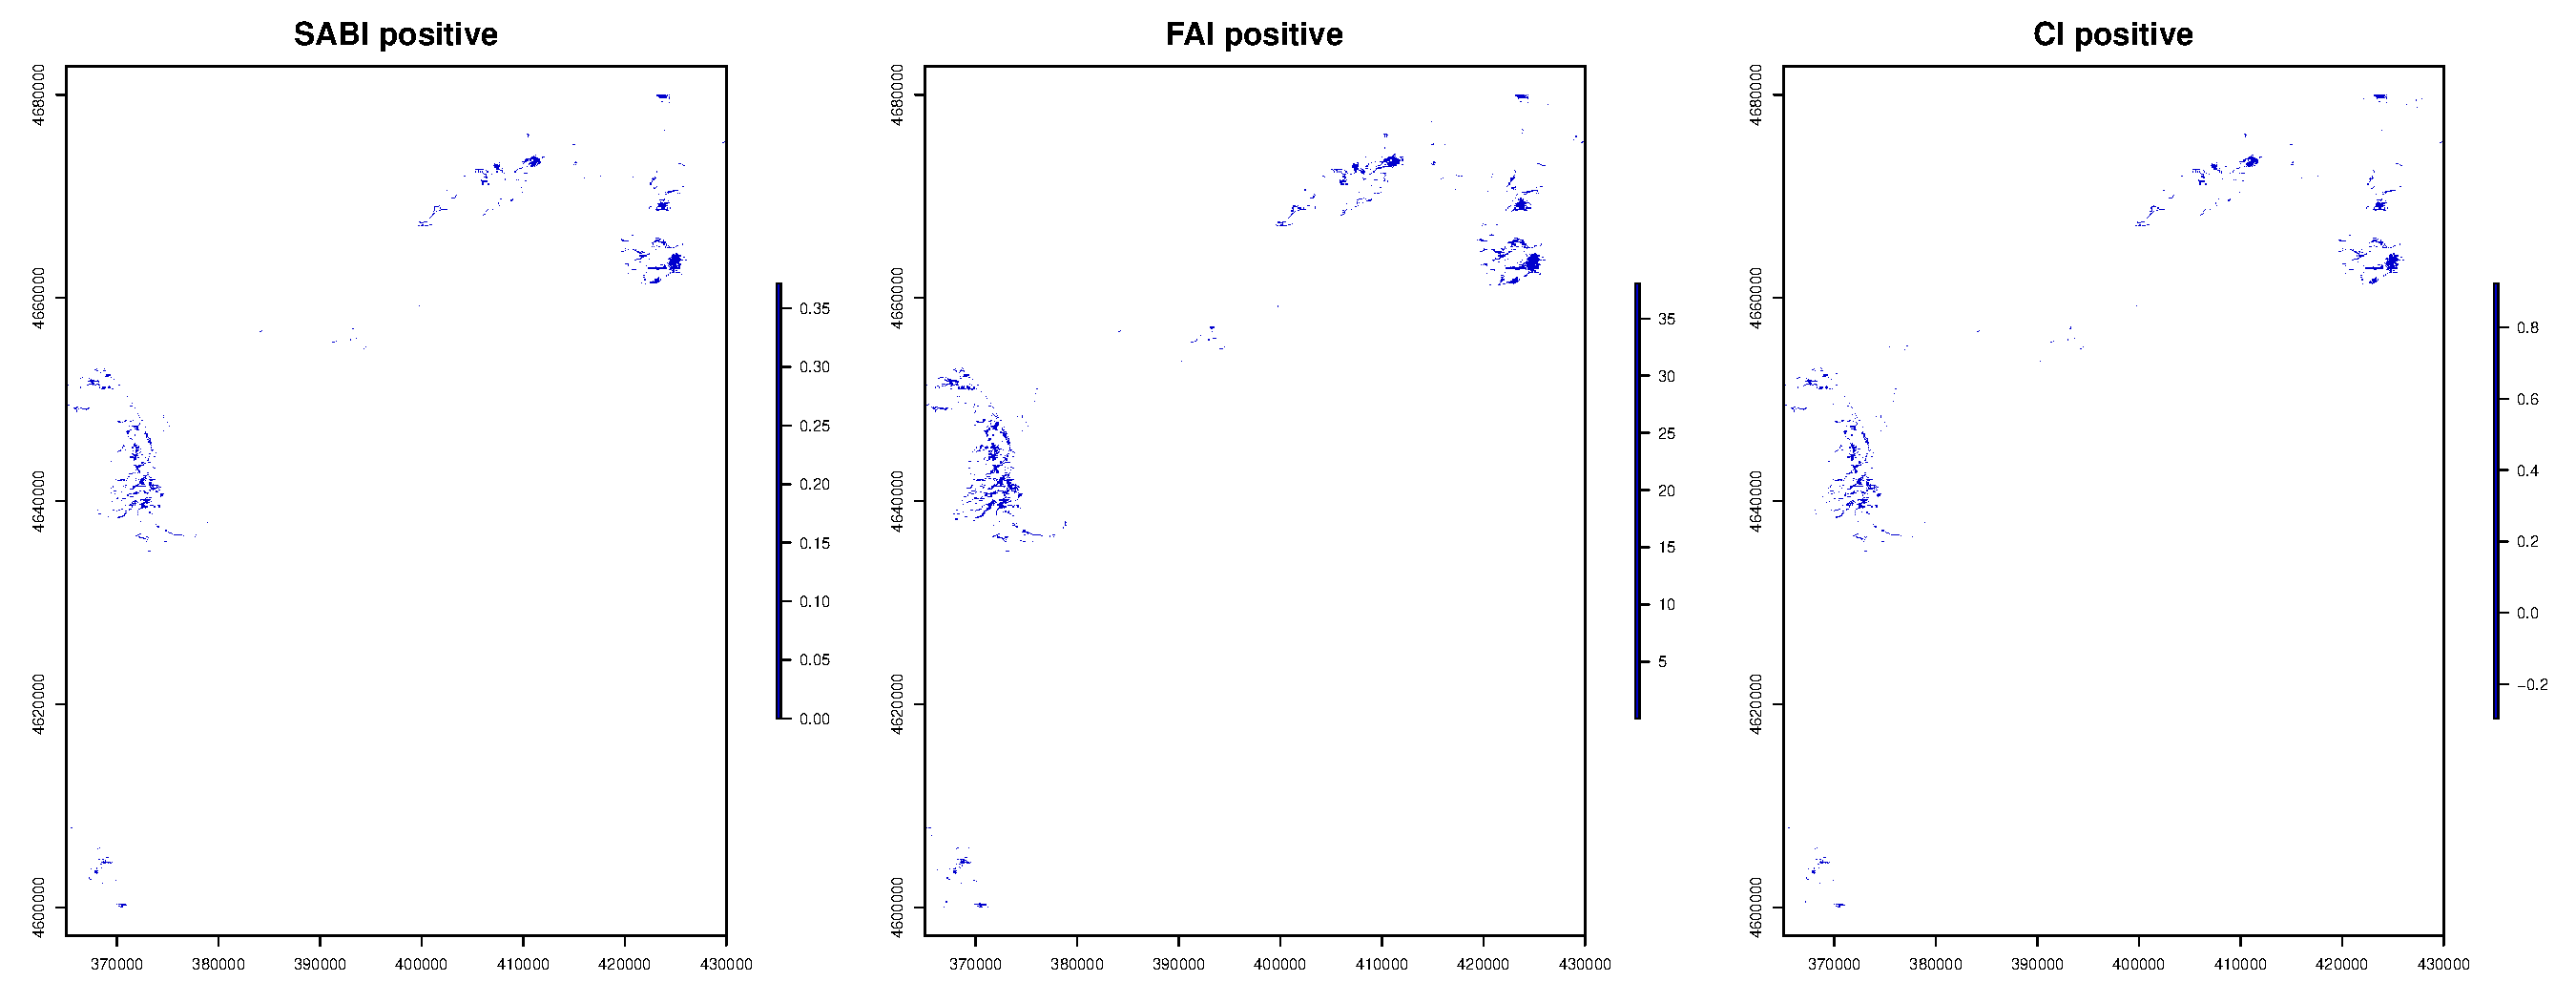
\includegraphics[width = 0.9\textwidth]{images/positive.pdf}
\end{figure}
\end{frame}

\begin{frame}[fragile]{Chlorophyll estimation}
\begin{lstlisting}[firstnumber = 78]
#create stack with the interesting indeces
ref <- stack(ci, sabi, fai)
dat2 <- as.data.frame(ref)

#delete NAN
dat2 <- na.omit(dat2)

#overlay density on histrograms
c1 <- ggplot(dat2, aes(x = layer.1)) +
  geom_histogram(aes(y = ..density..), color = "black", fill = "white", lwd = 0.5) + 
  geom_density(lwd = 1, fill = "aquamarine3", col = "aquamarine3", alpha = 0.25) +
  labs(title = "CI_distribution", x = "Value", y = "Density")   
\end{lstlisting}   
\end{frame}

\begin{frame}{}
 Same procedure for the others 2 indices. Then use \textit{\textbf{library(patchwork)}} to combine them in one image: \textit{\textbf{c1 + c2 + c3}}.
\begin{figure}
\centering
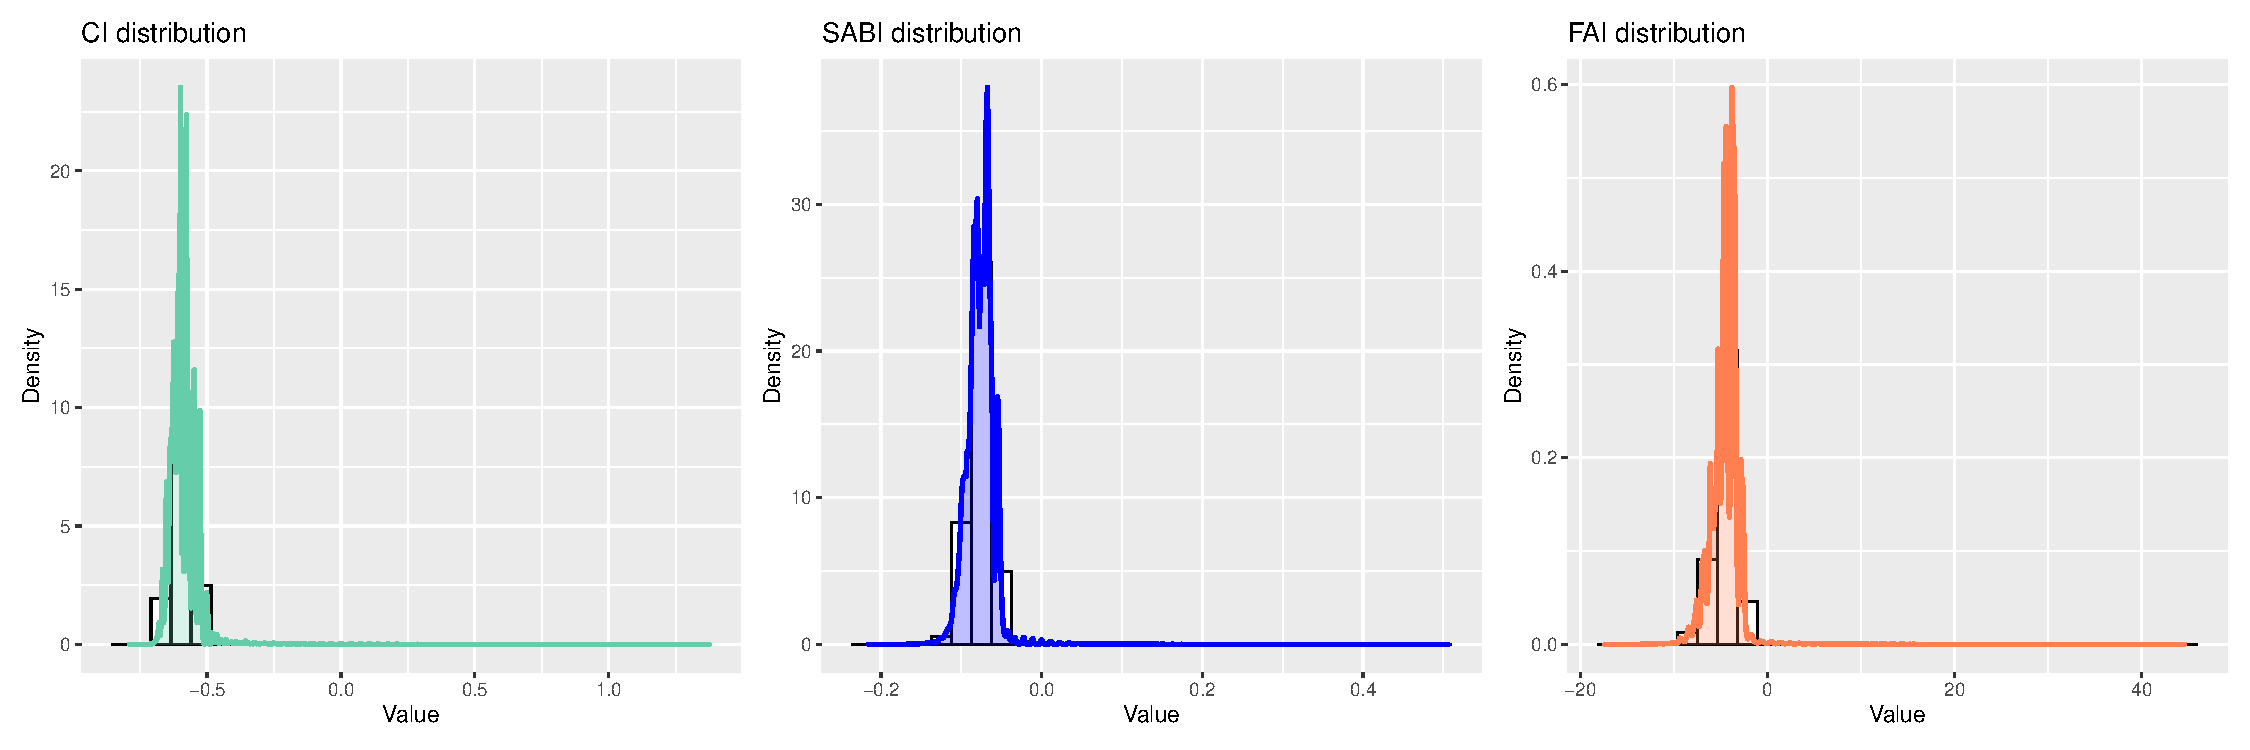
\includegraphics[width =\textwidth]{images/his_des.pdf}    
\end{figure}
\end{frame}

\section{Conclusions}
\begin{frame}{Final remarks}
\begin{itemize}
    \item To study floating algae are necessary \textbf{particular indices}. Using traditional vegetation indices can lead to wrong results.
    \item Floating algae do not have a strong emission in NIR or some \textbf{correction} to the calculation must be introduced due to the different environment.
    \item Areal extension of the algae bloom can be evaluated.
\end{itemize}
\end{frame}

\section{References}
\begin{frame}[allowframebreaks]{References}
\bibliography{bibl}
\bibliographystyle{unsrt}
%\addcontentsline{toc}{section}{References} 
\nocite{nasa}
\nocite{veg_index}
\nocite{article}
\nocite{inproceedings}
\nocite{chlorophyll}
\end{frame}

\end{document}
